\chapter{Incertezza strumentale e regole di scrittura}

\begin{figure}[h]
    \centering
    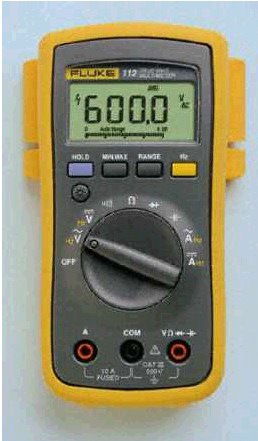
\includegraphics[scale = 1]{Fluke 112.png}
\end{figure}

\newpage 

\section{Il processo "reale" di misurazione}
\footnote{Slide della prof | SDME 2 Incertezza strumentale e regole di scrittura | pag 3 \\  
Appunti | 2025-03-12 | pag 6}

Di seguito la definizione di Misura data dalla norma UNI 4546: \newline

\textbf{Misura} : Informazione costituita da un valore, una incertezza ed una unità di misura, 
assegnata a presentare un parametro in un determinato stato del sistema. \newline 

Come si vede da un esempio di misura: 

\begin{figure}[h]
    \centering
    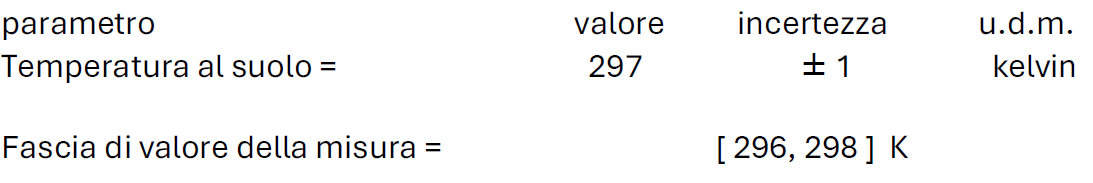
\includegraphics[scale = 0.5]{Esempio di misurazione.PNG}
\end{figure}

la misura è uno qualunque dei valori compresi nella fascia tra 297-1 kelvin e 297+1 kelvin. \newline 

\newpage 

\section{Incertezza degli strumenti di misura}
\footnote{Slide della prof | SDME 2 Incertezza strumentale e regole di scrittura | pag 4 \\  
Appunti | 2025-03-12 | pag 6 - 7}

Ciò che differisce il mondo ideale a quello reale è che 
gli strumenti di misura sono afflitti principalmente da tre effetti: 

\begin{itemize}
    \item Incertezza dei campioni negli strumenti 
    \item Deriva termica 
    \item Imprecisioni costruttive dello strumento 
\end{itemize}

Dalle specifiche degli strumenti, 
si ricava l'incertezza strumentale (in inglese accuracy). \newline 

Ad esempio, dalle specifiche del multimetro di questo multimetro Fluke 112: 

\begin{figure}[h]
    \centering
    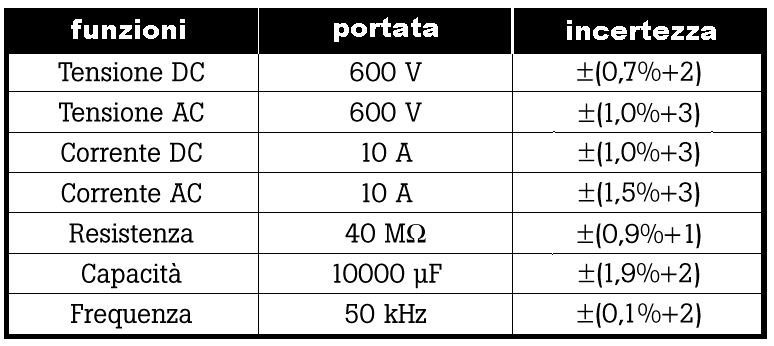
\includegraphics[scale = 0.5]{Specifiche Fluke 112.png}
\end{figure}

si nota nota che, nella colonna incertezza di questo strumento, l'incertezza è espressa in formula binomia. \newline 

Per formula binomia si intende una incertezza che è composta come: 

{
    \Large 
    \begin{equation}
        \pm (\text{ Percentuale del valore letto sul display} + \text{Numero digit})
    \end{equation}
}

La percentuale del valore letto sul display varia in base al valore che si legge sul display, 
invece il numero di digit è un contributo fisso. \newline 

Sempre dalla tabella delle specifiche tecniche del Fluke 112, possiamo notare che, 
per ogni tipologia di grandezza che lo strumento può misurare, il costruttore dichiara portata e accuracy con cui lo strumento opera. \newline 

\newpage 

\subsection{Incertezza dei campioni utilizzati}
\footnote{Slide della prof | SDME 2 Incertezza strumentale e regole di scrittura | pag 5 - 6 \\  
Appunti | 2025-03-12 | pag 7 - 8}

Gli strumenti utilizzano uno o più campioni di una grandezza all'interno del loro strumento per svolgere una misura. \newline 

Come riportato nel DataSheet dell'integrato AD587 dell'Analog Devices: 

\begin{figure}[h]
    \centering
    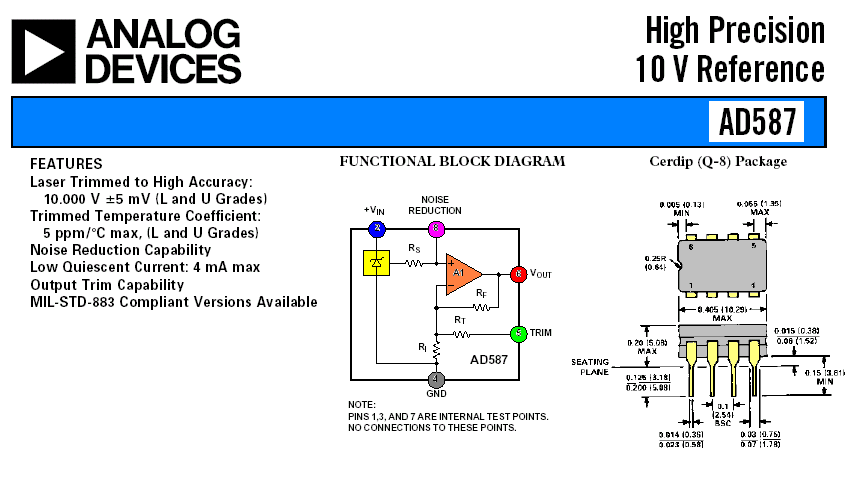
\includegraphics[scale = 0.5]{AD587 specs.png}
\end{figure}

l'integrato è un campione di riferimento di 10.000 V con incertezza di $\pm 5 \text{ } mV$. \newline 

Anche i campioni che materializzano le u.d.m. nei nostri strumenti sono affetti da incertezza (accuracy). \newline 

Tutte le misure che verranno fatte rapportando il valore della tensione incognita a questo valore campione saranno affette da alterazione ed essa sarà in parte proporzionale 
all'entità della tensione incognita stessa. \newline 

Si può corregge e minimizzare questa alterazione con la taratura. \newline 

O, in altri termini, l'incertezza proporzionale esiste perchè, generalmente, 
la misura viene fatta per confronto rispetto ad un riferimento, il quale ha a sua volta una sua incertezza. \newline 

\newpage 

\subsection{Deriva termica del campione}
\footnote{Slide della prof | SDME 2 Incertezza strumentale e regole di scrittura | pag 7 \\  
Appunti | 2025-03-12 | pag 8}

Come riportato nel DataSheet dell'integrato AD587 dell'Analog Devices, l'integrato di 10 V di riferimento è affetto da $5 \text{ } ppm/^{\circ} C $ max,
cioè il riferimento varierà massimo di 5 parti per milione per ogni grado centigrado. \newline 

A differenza dell'incertezza sul valore nominale, l'effetto della temperatura sul valore di tensione non può essere corretto con la taratura. \newline 

Si può eseguire la taratura per confronto con un campione di qualità superiore, a temperatura controllata, 
ma, a seguito della taratura, non si può garantire che la temperatura resti la stessa durante le operazioni di misura. \newline 

Basti banalmente capire la differenza e la stabilità della temperatura tra un laboratorio, dove la temperatura è controllata e stabile, 
e la temperatura "nel campo" di un tester. \newline 

\newpage 

\section{Imprecisioni costruttive dello strumento}
\footnote{Slide della prof | SDME 2 Incertezza strumentale e regole di scrittura | pag 8 - 9 \\  
Appunti | 2025-03-12 | pag 8}

Lo strumento è affetto anche esso dalla deriva termica, che, come sottolineato dalla deriva termica dei campioni, non si può modificare e/o 
calibrare con una taratura. \newline 

Ponendo ad esempio il tester Fluke 112, lo strumento contiene un campione di f.e.m. di 10 V, ma il costruttore dichiara una portata per le misure di tensione 
DC di 600 V. \newline

Ciò è possibile grazie a opportuni circuiti di confronto come, ad esempio, 
un partitore di tensione. \newline 

Come studiato dall'Elettrotecnica (mitico Stefano Squartini), 
un partitore di tensione è un circuito composto da due o più resistori in serie come in figura: 

\begin{figure}[h]
    \centering
    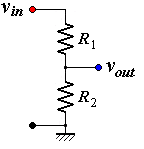
\includegraphics[scale = 1]{Partitore di tensione con due resistori.png}
\end{figure}

Sapendo i valori dei due resistori, cioè:

{
    \Large 
    \begin{equation} 
        \begin{cases}
            R_1 = R_{1 \text{nominale}} + \delta R_1
            \\ 
            R_2 = R_{2 \text{nominale}} + \delta R_2
        \end{cases}
    \end{equation}
}

dove $\delta R_1$ e $\delta R_2$ sono le tolleranze dei resistori reali rispetto ai valori nominali. \newline 

Sempre dall'Elettrotecnica, la tensione di uscita $v_{out} (t)$ sarà: 

{
    \Large 
    \begin{equation}
        v_{out} (t)
        = 
        \frac{R_2}{R_1 + R_2} v_{in} (t)
    \end{equation}
}

Essendo: 

{
    \Large 
    \begin{equation}
    \frac{R_2}{R_1 + R_2} < 1       
    \end{equation}
}

la tensione di ingresso $v_{in} (t)$ sarà diminuita: questo coefficiente prende il nome di rapporto di partizione 
e viene utilizzato dai costruttori di strumenti per confrontare la tensione di ingresso con la tensione di riferimento, i quali possono differire di diversi ordini di grandezza. \newline 

Aggiungendo anche le tolleranze dei due resistori, possiamo esprimere $v_{out} (t)$ come: 

{
    \Large 
    \begin{equation}
        v_{out} (t)
        = 
        \frac{R_{2 \text{nominale}} + \delta R_2}{ R_{1 \text{nominale}}+ R_{2 \text{nominale}} + \delta R_1 + \delta R_2} v_{in} (t) 
    \end{equation}
}

I valori di $\delta R_1$ e $\delta R_1$ sono presenti anche nell'espressione di $ v_{out} (t)$, 
quindi anche  $ v_{out} (t)$ varierà a causa della temperatura. \newline 

Sempre dall'espressione di  $ v_{out} (t)$, l'alterazione agisce in modo proporzionale. \newline 

Come scritto precedentemente, per ovviare alle imprecisioni costruttive dello strumento 
si possono tarare i campioni di riferimento delle grandezze, in genere il campione di f.e.m. . \newline 

La taratura e la certificazione dal LAT aggiungono un costo economico allo strumento di misura, 
come si vede da questo screenshot di un negozio online di strumenti di misura: 

\begin{figure}[h]
    \centering
    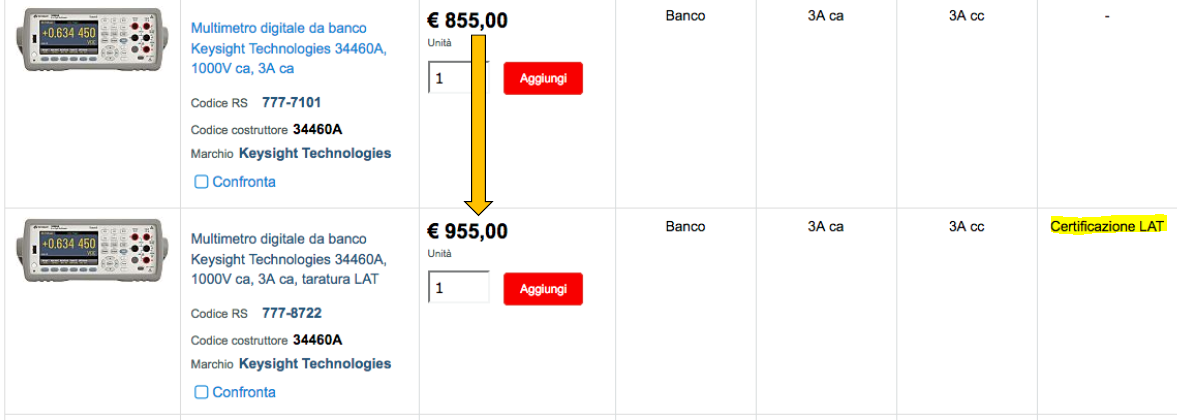
\includegraphics[scale = 0.5]{Confronto tra strumenti di misura con e senza certifiazione LAT.PNG}
\end{figure}


\newpage 

\subsection{Deriva termica dell'Offset degli OpAmp}
\footnote{Slide della prof | SDME 2 Incertezza strumentale e regole di scrittura | pag 10 \\  
Appunti | 2025-03-12 | pag 8}

All'interno degli strumenti di misura, sono inseriti gli amplificatori operazioni, 
strumenti non lineari inseriti per svolgere dei calcoli matematici (capirete meglio in futuro quando discuteremo delle architetture degli strumenti). \newline 

\begin{tcolorbox}

    Vi lascio dei video per rinfrescare la memoria su cosa sono gli amplificatori operazioni (detti e abbreviati in inglese OpAmp) dal corso di Elementi di Elettronica: 
    \begin{itemize}
        \item EEVblog \# 600 - OpAmps Tutorial - What is an Operational Amplifier?\\ \url{https://youtu.be/7FYHt5XviKc?si=4V3S8tFyC56y07hG} 
        \item What is an operational amplifier? - by Khan  Academy\\ \url{https://youtu.be/lJDjWZqhpVc?si=MouXEfN111w36XkM} 
    \end{itemize}

    Un fenomeno molto importante degli OpAmp è quello della massa virtuale (virtual ground in inglese), spiegati in questi video: 
    \begin{itemize}
        \item Virtual ground - by  by Khan  Academy\\ \url{https://youtu.be/pxKLeIjzxAk?si=qQZbF8nnEPm39s_I} 
        \item Guest Video: Bob DuHamel - How Opamp Virtual Grounds Work\\ \url{https://youtu.be/HbMnQdRzD8A?si=j4Np3j3G4TOOuCNx} 
    \end{itemize}

    L'ultimo video l'ho lasciato solo per il meme e perchè aveva una copertina alquanto bizzarra. \newline 
    Tutti i video sono disponibili con le traduzioni automatiche in Italiano di Youtube
\end{tcolorbox}

Il problema maggiore dei OpAmp nel mondo fisico reale (o come scrivono i Gen Z su internet, in IRL), è che sono affetti, anche loro, dalla deriva termica. \newline 

Le derive termiche, come scritto precedentemente, non possono essere corretti con la taratura. \newline 

Ad esempio dalla configurazione invertente di OpAmp come in figura: 

\begin{figure}[h]
    \centering
    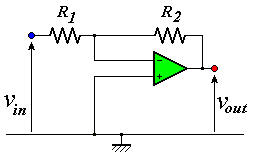
\includegraphics[scale = 1]{Configurazione invertente di un OpAmp.png}
\end{figure}

dove, si dimostra (cioè non lo dimostriamo) che la tensione $v_{out} (t)$ è: 

{
    \Large 
    \begin{equation}
        v_{out} (t) = - \frac{R_2}{R_1} v_{in} (t)
    \end{equation}
}

Nella realtà, dovremmo modellare il precedente in questa maniera: 

\begin{figure}[h]
    \centering
    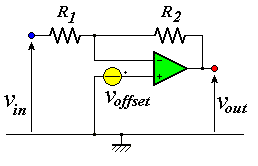
\includegraphics[scale = 1]{Configurazione invertente di un OpAmp reale.png}
\end{figure}

\newpage 

dove, rispetto al caso ideale, è presente una tensione di offset $V_{offset}$. \newline 

La tensione $V_{out}$ in uscita sarà: 

{
    \Large 
    \begin{equation}
        v_{out} (t) = - \frac{R_2}{R_1} 
        \left[ v_{in} (t) - v_{offset} (\theta) \right]
    \end{equation}
}

Nella realtà, le imperfezioni costruttive fanno nascere un contributo alla tensione di uscita dovuto alla temperatura (che abbiamo espresso nella funzione di $v_{out}$ con il simbolo $\theta$) 
che schematizzano con la nascita di una tensione di offset. \newline 

Per tensione di offset si intende che se $V_{in}$ è nulla, a $V_{out}$ sarà presente una tensione, che è uguale a $v_{offset}$. \newline 

\begin{tcolorbox}
    Se vuoi approfondire perchè si genera una tensione di offset all'ingresso di un OpAmp, ti lascio il seguente video: \newline 
    Offset voltage in op-amps (Amplifiers \# 8) - by Aaron Danner \\ \url{https://www.youtube.com/watch?v=biZ30H4bhks} \newline 

    In breve, la tensione di offset è dovuto alla rete circuitale dell'OpAmp
\end{tcolorbox}

\newpage 

\section{Perturbazione dello stato del sistema}
\footnote{Slide della prof | SDME 2 Incertezza strumentale e regole di scrittura | pag 11-12 \\  
Appunti | 2025-03-12 | pag 9 | 2025-04-14 | pag 2 - 3}

Nel caso ideale, se volessimo misurare la tensione ai capi di un generatore di tensione, 
lo schema circuitale sarebbe quello seguente: 

\begin{figure}[h]
    \centering
    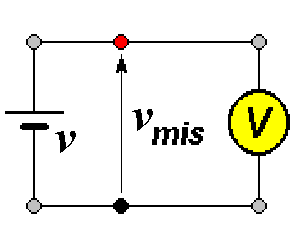
\includegraphics[scale = 0.6]{Tensione misurata caso ideale.png}
\end{figure}

Grazie all'elettrotecnica, nella realtà, una batteria stilo che "compriamo al supermercato" come quella in figura: 

\begin{figure}[h]
    \centering
    
\includegraphics[scale = 0.2]{Batteria duracell.jpg}
\end{figure}

ha una sua rappresentazione che non sarà un generatore indipendente di tensione, 
bensì sarà un generatore indipendente di tensione con in serie una resistenza di Thevenin. \newline 

\begin{tcolorbox}
    Se serve un piccolo ripasso su cosa è la rappresentazione di Thevenin, 
    puoi vedere il seguente video: \newline 
    Elettrotecnica - Lezione 14 - Equivalente di Thevenin e Norton - di Elettronicamente\\ \url{https://youtu.be/cyw17JX1sd4?si=nsyMihd74wiDm8JG}
\end{tcolorbox}

Il nuovo circuito di misura sarà il seguente: 

\begin{figure}[h]
    \centering
    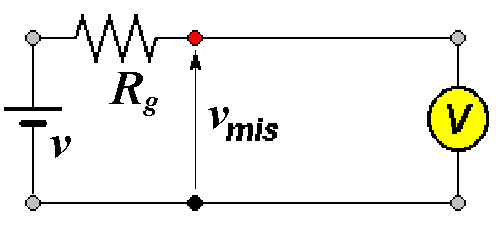
\includegraphics[scale = 0.6]{Circuito di misura con rappresentazione di Thevenin.png}
\end{figure}

Quindi, se la tensione misurata non sarà la tensione ai capi del generatore di tensione, bensì: 

{
    \Large 
    \begin{equation}
        \begin{cases}
            v_{mis} = v - v_{R_{g}} 
            \\ 
            v_{mis} \neq v
        \end{cases}
    \end{equation}
}

dove $v_{R_{g}}$ è la tensione ai capi del resistore $R_g$. \newline 

Per riassumere, la tensione che andremo realmente a misurare non sarà quella a vuoto del generatore, 
ma quella "sotto carico" ovvero la $v_{mis}$. \newline 

Per modellare un voltmetro reale, si pone la sua resistenza $R_v$ in parallelo ad esso.\newline 

Il nuovo circuito di misura sarà il seguente: 

\begin{figure}[h]
    \centering
    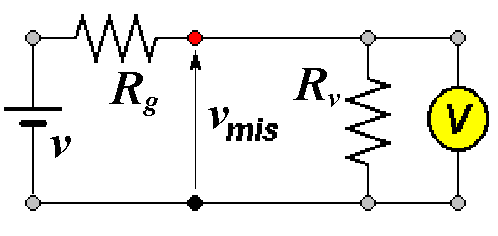
\includegraphics[scale = 0.6]{Circuito di misura con rappresentazione di Thevenin e Norton.png}
\end{figure}

In un voltmetro ideale, lo strumento è caratterizzato da impedenza di ingresso $R_v$ infinita 
che non viene attraversata da nessuna corrente. \newline 

In un voltmetro reale, lo strumento ha una sua impedenza $R_v$ in cui scorre corrente: 
lo strumento diventa un partitore di tensione. \newline 

La tensione che realmente misureremo sarà: 

{
    \Large 
    \begin{equation}
        \begin{cases}
            v_{mis}
            = 
            v \frac{R_v}{R_g + R_v} 
            \\ 
            v_{mis}
            \neq 
            v
        \end{cases}
    \end{equation}
}

A causa di questa $R_v$ del voltmetro reale, avviene una perturbazione del sistema. \newline 

Possiamo calcolare $\delta v$, cioè la differenza tra la tensione misurata e quella ideale, come: 

{
    \Large 
    \begin{equation}
        \begin{split}
            \delta v
            &= 
            v_{mis} - v 
            \\ 
            &= 
            v \frac{R_v}{R_g + R_v} - v 
            \\
            &= 
            - \frac{R_v}{R_g + R_v} v
        \end{split}
    \end{equation}
}

$\delta v$ è di segno negativo, quindi si sottostimerà la tensione $v_{mis}$. \newline 

Se svolgiamo il rapporto tra $\delta v$ e v abbiamo: 

{
    \Large 
    \begin{equation}
        \frac{\delta v}{v}
        = 
        - \frac{R_v}{R_g + R_v}
    \end{equation}
}

Se $R_v >>> R_g$, cioè $R_v$ è molto più grande rispetto a $R_g$, 
il denominatore di $\frac{\delta v}{v}$ tenderà a zero e/o diminuirà di molto. \newline 

\newpage 

\section{Disturbi e rumori elettrici, magnetici ed elettromagnetici}
\footnote{Slide della prof | SDME 2 Incertezza strumentale e regole di scrittura | pag 13 \\  
Appunti | 2025-03-14 | pag 3}

Nel mondo fisico e reale in cui viviamo, possono verificarsi dei disturbi elettromagnetici non voluti. \newline 

In base alla frequenza che vogliamo misurare, possiamo utilizzare questo grafico per rappresentare 
quanto il disturbo elettromagnetico impatta la misura: 

\begin{figure}[h]
    \centering
    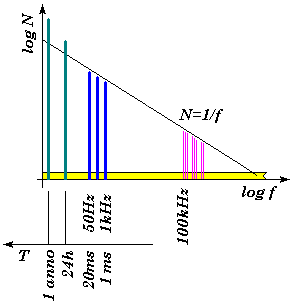
\includegraphics[scale = 0.8]{Disturbi elettromagnetici in base alla frequenza.png}
\end{figure}

I disturbi elettromagnetici sono causati da dispositivi non lineari. \newline 

Generalmente, i dispositivi di misura sono protetti da questi disturbi, ma è sempre meglio a priori accorgersi 
e prendere degli accorgimenti riguardo i disturbi elettromagnetici presenti nell'ambiente in cui si vuole fare la misura, 
perchè, oltre alla grandezza che si vuole misurare, misureremo anche il disturbo stesso, che si sommerà alla grandezza da misurare. \newline 

Inoltre, i disturbi sono difficili da identificare. \newline 

Ritornando alla figura dei disturbi di rete e delle armoniche generate dai dispositivi non lineari (cioè la figura sovrastante), 
se si vuole misurare una grandezza per 1 anno o 24 ore, la misura sarà afflitta da disturbi dovute alla derive termiche. \newline 

I disturbi a 50 Hz e 1 kHz sono dovuti alla rete elettrica, in particolare agli interruttori switching presenti nei dispositivi che abbiamo in casa. \newline 

Invece, i disturbi ad alta frequenza, cioè oltre i 100 kHz, sono dovuti alle radiocomunicazioni e al rumore termico. \newline 

La riga gialla indica il rumore termico che è AWGN (Additive White Gaussian Noise), cioè a spettro piatto e presente in tutte le frequenze. \newline 

\newpage 

\section{Incertezza strumentale: bit e digit}
\footnote{Slide della prof | SDME 2 Incertezza strumentale e regole di scrittura | pag 14 \\  
Appunti | 2025-03-14 | pag 4}

Visto che oramai ogni giorno abbiamo a che fare con uno strumento di misura digitale, 
lo strumento ci mostra, generalmente sul suo display, diverse cifre. \newline 

Siccome questi strumenti digitali contengono dei registri, ogni numero sarà 
rappresentato e interpretato dalla circuiteria come una serie di valori binari. \newline 

Per esempio il numero in decimale 149, in binario diventa: 
{
    \Large
    \begin{equation}
        149_{10} 
        \to 
        1001\text { } 0101_{2}
    \end{equation}
}

Si può fare anche il processo inverso, partendo dalla cifra più a sinistra e andando verso destra: 

{
    \Large 
    \begin{equation}
        \begin{split}
        1001\text { } 0101 
        &= 
        2^{7} + 2^{4} + 2^{2} + 2^{0} 
        \\ 
        &= 
        128 + 16 + 4 + 1 
        \\ 
        &= 
        149
        \end{split}
    \end{equation}
}

\begin{tcolorbox}
    Se vuoi ripassare un po' le conversioni tra le basi numeriche: \newline 
    \url{https://www.youmath.it/domande-a-risposte/view/8207-da-decimale-a-binario.html}
\end{tcolorbox}

Quindi, il primo bit, quello più a destra viene nominato come LSB (Least Significant Bit), 
invece l'ultimo bit, quello più a sinistra, viene definito come MSB (Most Significant Bit). \newline 

Prendono questo nome, proprio perchè, come visto dalla conversione del numero digitale a quello decimale, 
i bit più a sinistra hanno un peso maggiore rispetto quelli a destra. \newline 

In questo caso $2^{7} > 2^{0}$. \newline 

Lo stesso principio dei pesi dei bit in base al loro ordine, lo si può applicare alle cifre che ci vengono fornite dallo strumento di misura. \newline 

In questo caso non si descriveranno i bit bensì i digit. \newline 

In figura un esempio di valori in un voltmetro e del suo display: 

\begin{figure}[h]
    \centering
    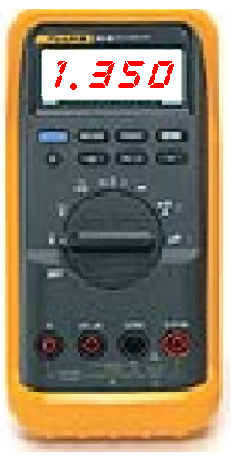
\includegraphics[scale = 0.6]{Digits in un voltmetro.PNG}
\end{figure}

\newpage 

La cifra 0 che si trova a destra viene definita LSD (Least Significant Digit), 
invece la cifra 1 che si trova a sinistra viene definita come MSD (Most Significant Digit). \newline 

\newpage 

\subsection{Espressione della incertezza degli strumenti indicatori (accuracy) - il "digit"}
\footnote{Slide della prof | SDME 2 Incertezza strumentale e regole di scrittura | pag 15 \\  
Appunti | 2025-03-14 | pag 4 - 5}

Se, ad esempio, abbiamo nel display del nostro strumento le cifre: 

{
    \Large 
    \begin{equation}
        1.350 \text{ [V]}
    \end{equation}
}

La formula simbolica per il calcolo dell'accuracy è la seguente: 

{
    \Large 
    \begin{equation}
        \Delta g \text{ } = \pm (a \% \text{ lettura }+ b \text{ digit }) 
    \end{equation}
}

Se dal produttore del voltmetro abbiamo la seguente indicazione del calcolo dell'accuracy: 

{
    \Large 
    \begin{equation}
        \Delta g \text{ } = \pm (1 \% \text{ lettura }+ 2 \text{ digit }) 
    \end{equation}
}

Generalmente la GUM consiglia 1 o 2 digit per il calcolo dell'accuracy. \newline 


Calcoliamo la prima parte dell'accuracy: 

{
    \Large 
    \begin{equation}
        \begin{split}
            \Delta g_{\text{lettura}}
            &= 
            1.350 \text{ [V]} 
            \cdot 1 \% 
            \\ 
            &= 
            0.0135 \text{ [V]}
        \end{split}
    \end{equation}
}

Considerando 2 digit, significa che da $\Delta g_{\text{lettura}}$ si considerano, 
partendo da sinistra andando verso destra, 2 cifre diverse da zero. \newline 

Quindi, $\Delta g_{\text{lettura}}$ diventa: 

{
    \Large 
    \begin{equation}
        \Delta g_{\text{lettura}} = 0.013
    \end{equation}
}

oppure, per notazione, si può anche scrivere le cifre che non comprendono i digit in minuscolo. \newline 

In questo particolare caso è valida anche la seguente notazione: 

{
    \Large 
    \begin{equation}
        \Delta g_{\text{lettura}} = 0.013_{5}
    \end{equation}
}

perchè il valore 5 è quel valore intermedio nell'intervallo. \newline 

Il valore 5 generalmente si arrotonda per eccesso, ma, scritto in questa maniera, si lascia all'utente finale se svolgere l'arrotondamento per eccesso o meno. \newline 

Siccome si considerano 2 digit, il secondo digit diverso da zero esprime 1 [mV], quindi: 

{
    \Large 
    \begin{equation}
        \begin{split}
            \Delta g_{\text{digit}} 
            &= 
            2 \cdot 1 \text{ [mV]}
            \\ 
            &= 
            2 \text{ [mV]}
        \end{split}
    \end{equation}
}

Combinando i due fattori $\Delta g_{\text{lettura}}$ e $\Delta g_{\text{digit}} $, 
si può esprimere $\Delta g$ come: 

{
    \Large 
    \begin{equation}
        \begin{split}
            \Delta g 
            &= 
            \pm 
            (\Delta g_{\text{lettura}} + \Delta g_{\text{digit}} ) \text{ [V]} 
            \\
            &=
            \pm 
            (0.0135_{5} + 0.002) \text{ [V]}
        \end{split}
    \end{equation}
}

Questo è un caso particolare perchè l'ultimo digit di $\Delta g_{\text{lettura}}$ è uguale a 5, 
quindi si va alla cifra superiore: 

{
    \Large 
    \begin{equation}
        \begin{split}
            &= 
            \pm 
            0.01_{55} \text{ [V]}
            \\ 
            &= 
            \pm 
            0.02 \text{ [V]}
        \end{split}
    \end{equation}
}

$\Delta g \text{ }= \text{ } \pm 0.02 \text{ [V]} $ è il valore di a, 
dalla quale si calcola l'incertezza di tipo B ipotizzando una pdf (densità di probabilità) dello strumento stesso. \newline 

\newpage 

\section{Riduzione della incertezza strumentale}
\footnote{Slide della prof | SDME 2 Incertezza strumentale e regole di scrittura | pag 16 \\  
Appunti | 2025-03-14 | pag 6}

Dalla definizione di misura della GUM, la misura è un processo, quindi anche la riduzione dell'incertezza è un processo. \newline 

Per ridurre l'incertezza, si possono applicare le seguenti accortezze: 

\begin{itemize}
    \item Periodicamente effettuare o richiedere la taratura dello strumento 
    \item Non eseguire misurazioni durante la fase di riscaldamento dello strumento, cioè non prima che sia superato il transitorio, perchè lo strumento è stato tarato ad una temperatura di riferimento che è quella di regime 
    \item Se si conoscono i parametri del sistema, si può calcolare la perturbazione dello stato del sistema provocata dallo strumento
\end{itemize}


Per quanto riguarda l'ultima accortezza, 
da un punto di vista analitico, 
dobbiamo determinare l'incertezza strumentale (cioè l'accuracy), 
se si ipotizza la pdf, per trovare la $u_{B} (x)$, 
che andrà combinata con la $u_{A} (x)$ e moltiplicata per un opportuno fattore di copertura k, per trovare U(x). \newline 

\newpage 

\section{Espressione della incertezza di misura}
\footnote{Slide della prof | SDME 2 Incertezza strumentale e regole di scrittura | pag 17 \\  
Appunti | 2025-03-14 | pag 6}

L'accuracy $\Delta g$ non solo può essere espressa nella formula scritta precedentemente, ma anche in altri modi. \newline 

Di seguito alcuni esempi. \newline 

\textbf{Incertezza assoluta} 

L'incertezza assoluta è l'ampiezza dell'intervallo centrato sul valore indicato x. \newline 

Si esprimere come: 

{
    \Large 
    \begin{equation}
        \Delta x = \pm \text{ } U
    \end{equation}
}


L'incertezza assoluta è dotata di dimensioni omogenee (cioè le stesse) alla grandezza sotto misura. \newline 

\textbf{Incertezza relativa} 

L'incertezza relativa è il rapporto fra i valori dell'incertezza assoluta $\Delta x$ e il valore indicato x. \newline 

Si esprime come: 

{
    \Large 
    \begin{equation}
        \frac{\Delta x}{x} 
        = 
        \pm 
        \frac{U}{x}
    \end{equation}
}

L'incertezza relativa, rispetto all'incertezza assoluta, è adimensionale. \newline 

Da un punto di vista qualitativo, aiuta a capire se la misura è di buona qualità. \newline 

\textbf{Incertezza percentuale}

L'incertezza percentuale esprime il valore dell'incertezza relativa moltiplicato per 100. \newline 

Si esprime come: 

{
    \Large 
    \begin{equation}
        \Delta x \% = \pm 100 \cdot \left(\frac{U}{x}\right)
    \end{equation}
}

Utilizzata comunemente nei contesti di misura. \newline 

\textbf{Incertezza relativa in ppm}

L'incertezza relativa in ppm (cioè parti per milione) esprime il valore dell'incertezza relativa moltiplicata per 1 000 000. \newline 

Si esprime come: 

{
    \Large 
    \begin{equation}
        \frac{\Delta x}{x} (ppm) 
        = 
        \pm 1 \cdot 10^{6} \cdot \left(\frac{U}{x}\right)
    \end{equation}
}

\newpage 

\section{Regola di scrittura: cifre significative}
\footnote{Slide della prof | SDME 2 Incertezza strumentale e regole di scrittura | pag 18 -21 \\  
Appunti | 2025-03-14 | pag 6 - 9}

Poniamo come esempio i seguenti dati: 

{
    \Large 
    \begin{equation}
        \begin{cases}
            x = 123.456 89 \text{ [V]} 
            \\ 
            U = \pm 0.001 41 \text{ [V]}
        \end{cases}
    \end{equation}
}

dove, come scritto precedentemente, U è l'incertezza assoluta e x è il valore letto sul display dello strumento. \newline 

Quindi x appartiene al seguente intervallo: 

{
    \Large 
    \begin{equation}
        \begin{split}
            123.456 89 - 0.001 41 \text{ [V] }
            < 
            \text{ }
            &x 
            \text{ }
            < 
            123.456 89 + 0.001 41 \text{ [V] }
            \\
            123.455 48 \text{ [V] }
            < 
            \text{ }
            &x 
            \text{ }
            < 
            123.458 30 \text{ [V] }
        \end{split}
    \end{equation}
}

Da un punto di vista grafico: 

\begin{figure}[h]
    \centering
    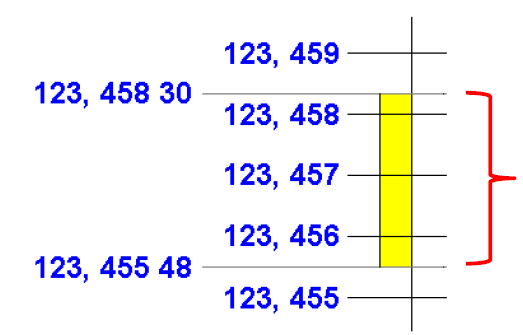
\includegraphics[scale = 0.5]{Intervallo di misura.PNG}
\end{figure}

Quella tratteggiata in rosso è la fascia dei valori della misurazione. \newline 

Ponendo la regola che ci dice la GUM, cioè esprimere l'incertezza 
con una o al massimo due cifre diverse da zero, e approssimando per eccesso, 
l'incertezza U diventa: 

{
    \Large 
    \begin{equation}
        \begin{split}
             U &= \pm 0.001 41 \text{ [V]}
             \\
             &\downarrow
             \\
             U &= \pm 0.002 \text{ [V]}
        \end{split}
    \end{equation}
}

Da un punto di vista grafico, non andremo a considerare l'intervallo precedente in giallo di prima, 
bensì quello verde che è più esteso:

\begin{figure}[h]
    \centering
    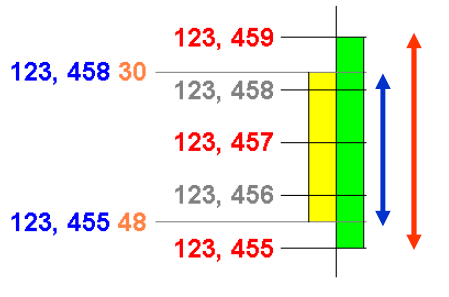
\includegraphics[scale = 0.5]{Intervallo di misura con approssimazioni.PNG}
\end{figure}


Inoltre, siccome abbiamo espresso l'incertezza, bisogna esprimere il valore centrale della misura. \newline 

Il valore centrale della misura diventa, 
applicando anche le approssimazioni e troncando alla stessa cifra dell'incertezza: 

{
    \Large 
    \begin{equation}
        \begin{split}
            x &= 123.456 89 \text{ [V]}
            \\ 
            &\downarrow 
            \\ 
            x &= 123.457 \text{ [V]}
        \end{split}  
    \end{equation}
}

Unendo il valore centrale e l'incertezza della misura insieme, 
la misura finale si può esprimere come: 

{
    \Large 
    \begin{equation}
        x = (123.457 \text{ } \pm \text{ } 0.002) \text{ [V]}
    \end{equation}
}

La regola aurea nelle misure è meglio esprimere una maggiore incertezza che una minore, 
e le incertezze vanno approssimate per eccesso, 
invece il valore medio al valore vicino. \newline 


\newpage 

\section{Compatibilità tra le misure}
\footnote{Slide della prof | SDME 2 Incertezza strumentale e regole di scrittura | pag 22 - 23 \\  
Appunti | 2025-03-14 | pag 9 - 10}

Un concetto molto importante dettate dalla GUM è quello di compatibilità. \newline

Essendo la misura un processo, due o più misure non possono essere uguali. \newline 

Al posto del concetto di uguaglianza, si sostituirà il concetto di compatibilità. \newline 

Diciamo che due misure di uno stesso misurando sono tra loro compatibili se gli intervalli dei valori "plausibili", 
ossia probabili ad un certo livello di confidenza che possono essere loro assegnati, 
hanno una adeguata sovrapposizione. \newline 

Da un punto di vista grafico: 

\begin{figure}[h]
    \centering
    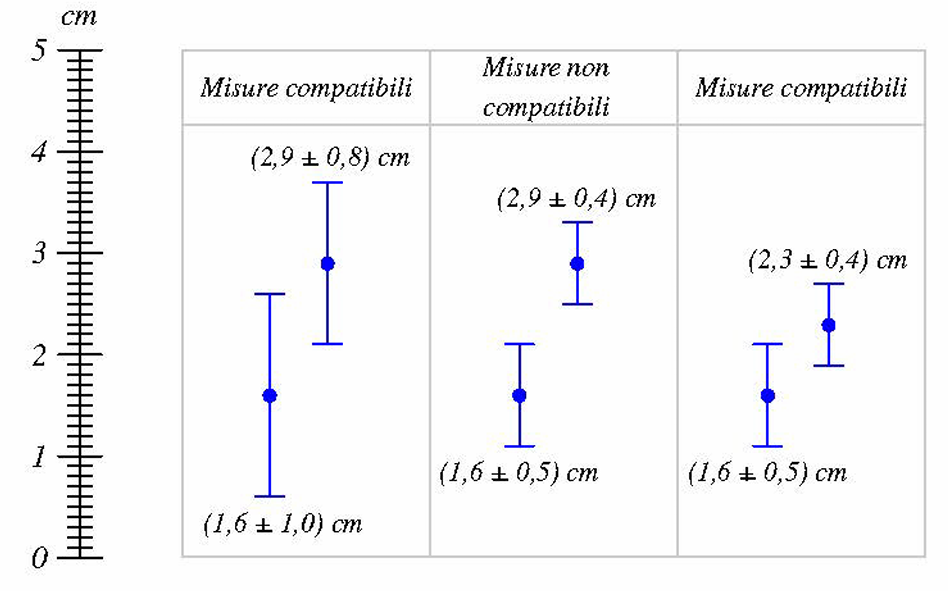
\includegraphics[scale = 0.3]{Esempio di misure compatibili.PNG}
\end{figure}

Per la definizione degli intervalli di compatibilità, 
è opportuno usare un adeguato fattore di ricopertura. \newline 

Il fattore di ricopertura lo indichiamo con la lettera a e deve essere: 

{
    \Large 
    \begin{equation}
        a \ge 1
    \end{equation}
}

a deve essere un numero intero. \newline

Nel caso di misure indipendenti, cioè non correlate, (quelle che studieremo in questo corso), 
la compatibilità si esprime come: 

{
    \Large 
    \begin{equation}
        \abs{x_1 - x_2} 
        \le 
        a \sqrt{u^{2}(x_1) + u^{2}(x_2)}
    \end{equation}
}

dove $x_1$ e $x_2$ sono i valori con le corrispettive incertezze $u(x_1)$ e $u(x_2)$. \newline 

Da un punto di vista pratico, 
normalmente si accetta la compatibilità se a ha un valore intero compreso tra: 

{
    \Large 
    \begin{equation}
        1 \leq a \leq 3
    \end{equation}
}


\newpage 

\subsection{Compatibilità tra le misure e media pesata}
\footnote{Slide della prof | SDME 2 Incertezza strumentale e regole di scrittura | pag 24 \\  
Appunti | 2025-03-14 | pag 10}

In presenza di un certo numero L di misure $x_1$, $x_2$, ..., $x_l$, ....., $x_L$ tra loro compatibili, 
il valore che si usa per esprimere il misurando è dato da una media pesata $\overline{x_{MP}}$ come: 

{
    \Large 
    \begin{equation}
        \begin{split}
            \overline{x_{MP}} 
            &= 
            \frac{\sum_{l=1}^{L} \frac{x_l}{u^{2} (x_l)}}
            {\sum_{l=1}^{L} \frac{1}{u^{2} (x_l)}}
            \\
            &= 
            \frac{\sum_{l=1}^{L} w_l x_l}
            {\sum_{l=1}^{L} w_l}
        \end{split}
    \end{equation}
}

dove: 

{
    \Large
    \begin{equation}
        w_l = \frac{1}{u^{2} (x_l)}
    \end{equation}
}

Dalla media pesata, si può calcolare il quadrato dell'incertezza stimata è data da: 

{
    \Large 
    \begin{equation}
        \begin{split}
            u^{2} (\overline{x_{MP}})
            &= 
            \frac{1}{\sum_{l = 1}^{L} \frac{1}{u^{2} (x_l)}}
            \\ 
            &= 
            \frac{1}{\sum_{l=1}^{L} w_l}
        \end{split} 
    \end{equation}
}

